\documentclass[
  bibliography=totoc,     % Literatur im Inhaltsverzeichnis
  captions=tableheading,  % Tabellenüberschriften
  titlepage=firstiscover, % Titelseite ist Deckblatt
]{scrartcl}

% Paket float verbessern
\usepackage{scrhack}

% Warnung, falls nochmal kompiliert werden muss
\usepackage[aux]{rerunfilecheck}

% unverzichtbare Mathe-Befehle
\usepackage{amsmath}
% viele Mathe-Symbole
\usepackage{amssymb}
% Erweiterungen für amsmath
\usepackage{mathtools}

% Fonteinstellungen
\usepackage{fontspec}
% Latin Modern Fonts werden automatisch geladen
% Alternativ:
%\setromanfont{Libertinus Serif}
%\setsansfont{Libertinus Sans}
%\setmonofont{Libertinus Mono}
\recalctypearea % Wenn man andere Schriftarten gesetzt hat,
% sollte man das Seiten-Layout neu berechnen lassen

% deutsche Spracheinstellungen
\usepackage{polyglossia}
\setmainlanguage{german}


\usepackage[
  math-style=ISO,    % ┐
  bold-style=ISO,    % │
  sans-style=italic, % │ ISO-Standard folgen
  nabla=upright,     % │
  partial=upright,   % ┘
  warnings-off={           % ┐
    mathtools-colon,       % │ unnötige Warnungen ausschalten
    mathtools-overbracket, % │
},                       % ┘
]{unicode-math}

% traditionelle Fonts für Mathematik
\setmathfont{Latin Modern Math}
% Alternativ:
%\setmathfont{Libertinus Math}

\setmathfont{XITS Math}[range={scr, bfscr}]
\setmathfont{XITS Math}[range={cal, bfcal}, StylisticSet=1]

% Zahlen und Einheiten
\usepackage[
locale=DE,                   % deutsche Einstellungen
separate-uncertainty=true,   % immer Fehler mit \pm
per-mode=symbol-or-fraction, % / in inline math, fraction in display math
]{siunitx}

% chemische Formeln
\usepackage[
version=4,
math-greek=default, % ┐ mit unicode-math zusammenarbeiten
text-greek=default, % ┘
]{mhchem}

% richtige Anführungszeichen
\usepackage[autostyle]{csquotes}

% schöne Brüche im Text
\usepackage{xfrac}

% Standardplatzierung für Floats einstellen
\usepackage{float}
\floatplacement{figure}{htbp}
\floatplacement{table}{htbp}

% Floats innerhalb einer Section halten
\usepackage[
section, % Floats innerhalb der Section halten
below,   % unterhalb der Section aber auf der selben Seite ist ok
]{placeins}

% Seite drehen für breite Tabellen: landscape Umgebung
\usepackage{pdflscape}

% Captions schöner machen.
\usepackage[
  labelfont=bf,        % Tabelle x: Abbildung y: ist jetzt fett
  font=small,          % Schrift etwas kleiner als Dokument
  width=0.9\textwidth, % maximale Breite einer Caption schmaler
]{caption}
% subfigure, subtable, subref
\usepackage{subcaption}

% Grafiken können eingebunden werden
\usepackage{graphicx}
% größere Variation von Dateinamen möglich
\usepackage{grffile}

% schöne Tabellen
\usepackage{booktabs}

% Verbesserungen am Schriftbild
\usepackage{microtype}

% Literaturverzeichnis
\usepackage[style=alphabetic,]{biblatex}
% Quellendatenbank
\addbibresource{lit.bib}

% Hyperlinks im Dokument
\usepackage[
  unicode,        % Unicode in PDF-Attributen erlauben
  pdfusetitle,    % Titel, Autoren und Datum als PDF-Attribute
  pdfcreator={},  % ┐ PDF-Attribute säubern
  pdfproducer={}, % ┘
]{hyperref}
% erweiterte Bookmarks im PDF
\usepackage{bookmark}

% Trennung von Wörtern mit Strichen
\usepackage[shortcuts]{extdash}

\title{V203: Verdampfungswärme und Dampfdruck-Kurve}
\author{
  Simon Schulte
  \texorpdfstring{
    \\
    \href{mailto:simon.schulte@udo.edu}{simon.schulte@udo.edu}
  }{}
  \texorpdfstring{\and}{, }
  Tim Sedlaczek
  \texorpdfstring{
    \\
    \href{mailto:tim.sedlaczek@udo.edu}{tim.sedlaczek@udo.edu}
  }{}
}
\publishers{TU Dortmund – Fakultät Physik}

\date{Durchführung: 29.11.2016\\
      Abgabe: 06.11.2016}


\begin{document}
\newpage
\maketitle
\tableofcontents
\newpage

\section{Zielsetzung}
\label{sec:zielsetzung}
In dem Versuch soll die Dampfdruckkurve von Wasser aufgenommen werden. Daraus
wird dann die Verdampfungswärme $L$ errechnet. Außerdem wird die
Temperaturabhängigkeit der Verdampfungswärme bestimmt.
\section{Theorie}
\label{sec:theorie}
Die drei Aggregatzustände von Wasser sind nicht absolut fest. So ist es bei
\SI{0}{\celsius} möglich, dass Wasser alle drei Aggregatzustände annimmt, also
sowohl fest, flüssig als auch gasförmig ist. Wenn man nun die Temperatur von
Wasser ändert und ein Inertialsystem erzeugt, in welchem man den Druck variieren
kann, ändert sich das Zustandsdiagramm von Wasser. In der Abbildung \ref{fig:aggregatzustände}
zu sehen ist das qualitative Zustandsdiagramm von Wasser.
\begin{figure}[htb]
  \centering
  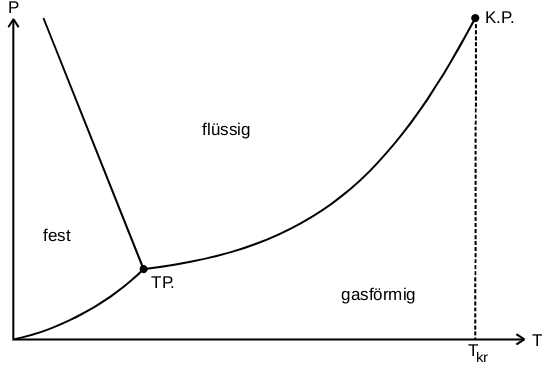
\includegraphics[width=0.8\textwidth]{Aggregatzustände.png}
  \caption{Qualitatives Zustandsdiagramm von Wasser \cite{anleitung}}
  \label{fig:aggregatzustände}
\end{figure}\\
Die Kurve von dem Punkt TP. zu K.P. nennt sich Dampfdruckkurve. Auf dieser
existieren zwei Aggregatzustände gleichzeitig, in diesem Fall flüssig und
gasförmig. Beim kritischen Punkt (K.P.) existiert kein Unterschied zwischen
flüssiger und gasförmiger Phase mehr. Der Verlauf dieser Kurve wird durch die
Verdampfungswärme $L$ festgelegt.

Um die Dampfdruckkurve eines Stoffes zu berechnen, nutzt man die Clausius-Clapeyronsche Gleichung:
\begin{equation}
  (V_D-V_F)\,\symup{d}\,p=\,\frac{L}{T}\,\symup{d}\,T
  \label{eqn:formel1}
\end{equation}
$V_D$, $V_F$ und $L$ sind Funktionen der Temperatur. $T$ ist die Temperatur
selbst und $p$ ist der Druck. Da bei der Integration der Clausius-Clapeyronschen
Gleichung $V_D$, $V_F$ und $L$ mitunter sehr kompliziert werden können, nähert
man diese folgendermaßen:
$V_F$ ist gegenüber $V_D$ vernachlässigbar, $V_D$ gehorcht der idealen
Gasgleichung
\begin{equation}
  V_D\,(p,\,T)\,=\,R\,\frac{T}{p}
  \label{eqn:formel2}
\end{equation}
und $L$ ist druck- und temperaturunabhängig. Dadurch ergibt sich für Gleichung
\eqref{eqn:formel1}
\begin{equation}
  \frac{R}{p}\,\symup{d}p\,=\,\frac{L}{T²}\,\symup{d}T
  \label{eqn:formel3}
\end{equation}
Wenn man dies nun integriert ergibt sich
\begin{equation}
  ln \left( p \right)\,=\,-\,\frac{L}{R}\,\cdot\frac{1}{T}\,+\,const
  \label{eqn:formel4}
\end{equation}
wobei $p$ der Druck ist, $R$ die allgemeine Gaskonstante und $L$
die Verdampfungswärme.
Die Allgemeine Gasgleichung ist gegeben durch:
\begin{equation}
  p\,\cdot\,V\,=\,n\,\cdot\,R\,\cdot\,T
  \label{eqn:formel5}
\end{equation}
Dabei ist $n$ die Stoffmenge in $\si{\mol}$.
\newpage
\section{Durchführung}
\label{sec:durchführung}
\subsection{Versuchsaufbau}
\label{sec:versuchsaufbau}
Die Apparatur für die Messungen im Druckbereich $p$ $\le$ \SI{1}{\bar} ist
wie in Abbildung \ref{fig:versuch1} aufgebaut.
Ein elektrisch beheizbarer Mehrhalskolben, gefüllt mit etwas Wasser, ist über
einen Rückflusskühler und eine Woulfsche Flasche mit einem Barometer und einer
Wasserstrahlpumpe verbunden. Der Rückflusskühler schützt das Barometer vor
Feuchtigkeit, indem aufsteigender Wasserdampf an ihm kondesieren kann. Die
Woulfsche Flasche schützt die Apparatur vor versehentlichem Eindringen kalten
Wassers durch die Wasserstrahlpumpe.
\begin{figure}[htb]
  \centering
  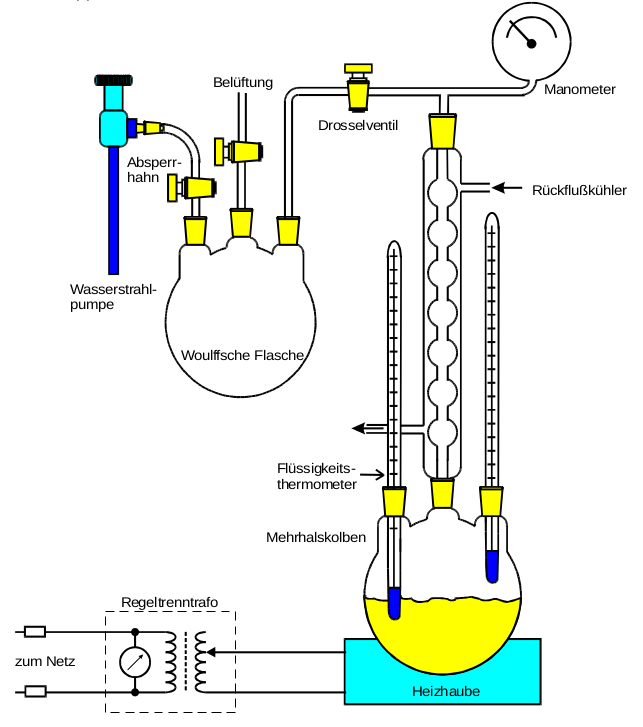
\includegraphics[width=0.8\textwidth]{Versuch1.png}
  \caption{Skizze der für den Druckbereich $p$\,$\le$\,\SI{1}{\bar} verwendeten Messapparatur \cite{anleitung}}
  \label{fig:versuch1}
\end{figure}\\
\\
Die Apparatur für die Messungen im Druckbereich \num{1}\,$<$\,$p$\,$\le$\,\SI{15}{\bar}
ist wie in Abbildung \ref{fig:versuch2} aufgebaut.
Die Wasserprobe befindet sich hierbei in einem Stahlzylinder, der, ebenfalls
elektrisch beheizt, weitaus höheren Drücken standhält. Dieser ist über ein
U-Rohr mit einem Drucksensor verbunden, welcher durch eine kleine Kühlschale mit
Wasser vor dem Überhitzen geschützt wird. Wie im ersten Aufbau ist auch hier ein
Thermometer in direkter Nähe zur Probe angebracht, wobei allerdings nun mit
einem digitalen Thermometer gearbeitet wird.
\begin{figure}[htb]
  \centering
  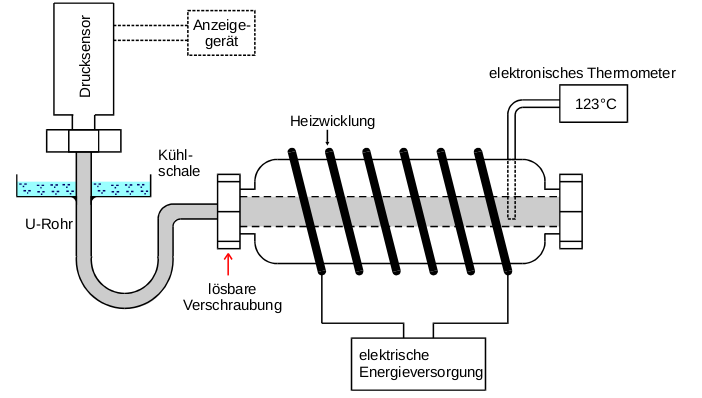
\includegraphics[width=0.8\textwidth]{Versuch2.png}
  \caption{Skizze der für den Druckbereich \num{1}\,$<$\,$p$\,$\le$\,\SI{15}{\bar} verwendeten Messapparatur \cite{anleitung}}
  \label{fig:versuch2}
\end{figure}
\subsection{Versuchsdurchführung}
\label{sec:versuchsdurcführung}
Das Experiment besteht aus zwei Teilversuchen. Im ersten Versuch wird die
Dampfdruckkurve von Wasser im Druckbereich zwischen \num{85} und
\SI{1000}{\milli\bar} ermittelt. Zunächst wird mithilfe der Wasserstrahlpumpe
die Glasapparatur evakuiert und der Innendruck somit soweit wie möglich gesenkt.
Danach werden alle Ventile geschlossen, der Rückflusskühler und die Heizhaube
werden eingeschaltet. Über das Thermometer, welches sich in der Dampfphase
oberhalb des Wassers befindet und das Barometer lassen sich, bei eingeschalteter
Heizhaube, laufend Wertepaare von Temperatur und Druck aufnehmen. Dabei wird in
\SI{5}{\milli\bar} Schritten zwischen \SI{85}{\milli\bar} und \SI{200}{\milli\bar}
gemessen und in \SI{50}{\milli\bar} Schritten zwischen \SI{200}{\milli\bar} und
\SI{1000}{\milli\bar} gemessen.\\
Wie im ersten Versuchsabschnitt wird die Probe beim zweiten Versuch kontinuierlich erhitzt, wobei
Temperatur- und Druckverlauf protokolliert werden. Gemessen wird nun im Druckbereich
zwischen \SI{1}{\bar} und \SI{15}{\bar}.
\section{Auswertung}
\label{sec:auswertung}
\subsection{Fehlerrechnung}
Die in der Auswertung verwendeten Mittelwerte mehrfach gemessener Größen sind
gemäß der Gleichung
\begin{equation}
    \bar{x}=\frac{1}{n}\sum_{i=1}^n x_i
    \label{eqn:formel6}
\end{equation}
bestimmt. Die Standardabweichung des Mittelwertes ergibt sich dabei zu
\begin{equation}
    \mathup{\Delta}\bar{x}=\sqrt{\frac{1}{n(n-1)}\sum_{i=1}^n\left(x_i-\bar{x}\right)^2}.
    \label{eqn:formel7}
\end{equation}
Resultiert eine Größe über eine Gleichung aus mehreren anderen fehlerbehafteten
Größen, so berechnet sich der Gesamtfehler nach der Gaußschen
Fehlerfortpflanzung zu
\begin{equation}
    \mathup{\Delta}f(x_1,x_2,...,x_n)=\sqrt{\left(\frac{\mathup{d}f}{\mathup{d}x_1}\mathup{\Delta}x_1\right)^2+\left(\frac{\mathup{d}f}{\mathup{d}x_2}\mathup{\Delta}x_2\right)^2+ \dotsb +\left(\frac{\mathup{d}f}{\mathup{d}x_n}\mathup{\Delta}x_n\right)^2}.
    \label{eqn:formel8}
\end{equation}

\subsection{Messwerte}
Für die beiden Versuche wurden die in Tabelle \ref{tab:messwerte} stehenden
Werte gemessen.\\
Außerdem wurden die folgenden Werte für die Allgemeine Gaskonstante R \cite{chemga} und die Avogadro-Konstante \cite{chemav}
$N_{\mathup{A}}$ verwendet:
\begin{equation}
  \mathup{R} = \SI{8.314}{\joule\per\mol\per\kelvin}
\end{equation}
\begin{equation}
  N_{\mathup{A}} = \SI{6.022e23}{\per\mol}
\end{equation}
\begin{table}
  \centering
  \caption{Messwerte.}
  \label{tab:messwerte}
  \sisetup{table-format=3.1}
  \begin{tabular}{S[table-format=1.3] S S[table-format=2.1] S}
    \toprule
    \multicolumn{2}{c}{Versuch 1 bis $\SI{1}{\bar}$} & \multicolumn{2}{c}{Versuch 2 über $\SI{1}{\bar}$}\\
    {$p \,/\, \si{\bar}$} & {$T \,/\, \si{\celsius}$} & {$p \,/\, \si{\bar}$} & {$T \,/\, \si{\celsius}$}\\
    \midrule
    0.085 & 22.5 & 3.4 & 132.0\\
    0.090 & 23.0 & 3.7 & 134.9\\
    0.095 & 24.5 & 4.0 & 137.5\\
    0.100 & 26.0 & 4.4 & 140.9\\
    0.105 & 27.5 & 4.6 & 142.5\\
    0.110 & 29.5 & 5.0 & 145.5\\
    0.115 & 31.0 & 5.4 & 148.4\\
    0.120 & 32.5 & 5.8 & 151.0\\
    0.125 & 34.0 & 6.0 & 152.3\\
    0.130 & 36.0 & 6.4 & 154.7\\
    0.135 & 38.0 & 6.6 & 155.8\\
    0.140 & 40.0 & 7.2 & 158.8\\
    0.145 & 41.5 & 7.4 & 160.1\\
    0.150 & 43.0 & 7.6 & 161.1\\
    0.155 & 44.5 & 8.0 & 163.0\\
    0.160 & 46.0 & 8.4 & 164.9\\
    0.175 & 49.5 & 8.6 & 165.8\\
    0.180 & 51.0 & 9.0 & 167.5\\
    0.185 & 52.0 & 9.4 & 169.2\\
    0.190 & 53.0 & 9.7 & 170.3\\
    0.195 & 53.5 & 10.0 & 171.5\\
    0.200 & 54.5 & 10.3 & 172.6\\
    0.250 & 63.0 & 10.9 & 174.4\\
    0.300 & 69.0 & 11.8 & 177.3\\
    0.350 & 72.5 & 12.3 & 178.6\\
    0.400 & 76.0 & 12.6 & 179.3\\
    0.450 & 78.5 & 12.9 & 179.9\\
    0.500 & 81.5 & 13.2 & 180.5\\
    0.550 & 84.0 & 13.6 & 181.2\\
    0.600 & 86.0 & 14.0 & 182.0\\
    0.650 & 88.0 & 14.7 & 183.0\\
    0.700 & 90.0 & 15.0 & 183.5\\
    0.750 & 92.0 &  & \\
    0.800 & 93.5 &  & \\
    0.850 & 95.5 &  & \\
    0.900 & 97.0 &  & \\
    0.950 & 98.5 &  & \\
    1.000 & 100.0 &  & \\
    \bottomrule
  \end{tabular}
\end{table}
\clearpage
\subsection{Messung unter $\SI{1}{\bar}$}
Zunächst soll der Logarithmus des Druckverhältnisses $ln \left( \frac{p}{p_0} \right)$ gegen die reziproke Temperatur $\frac{1}{T}$
aufgetragen werden. Dazu wird dann eine Ausgleichsgerade bestimmt und diese über einen Koeffizientenvergleich mit Formel \eqref{eqn:formel4}
verglichen, um L zu bestimmen.
\begin{figure}
  \centering
  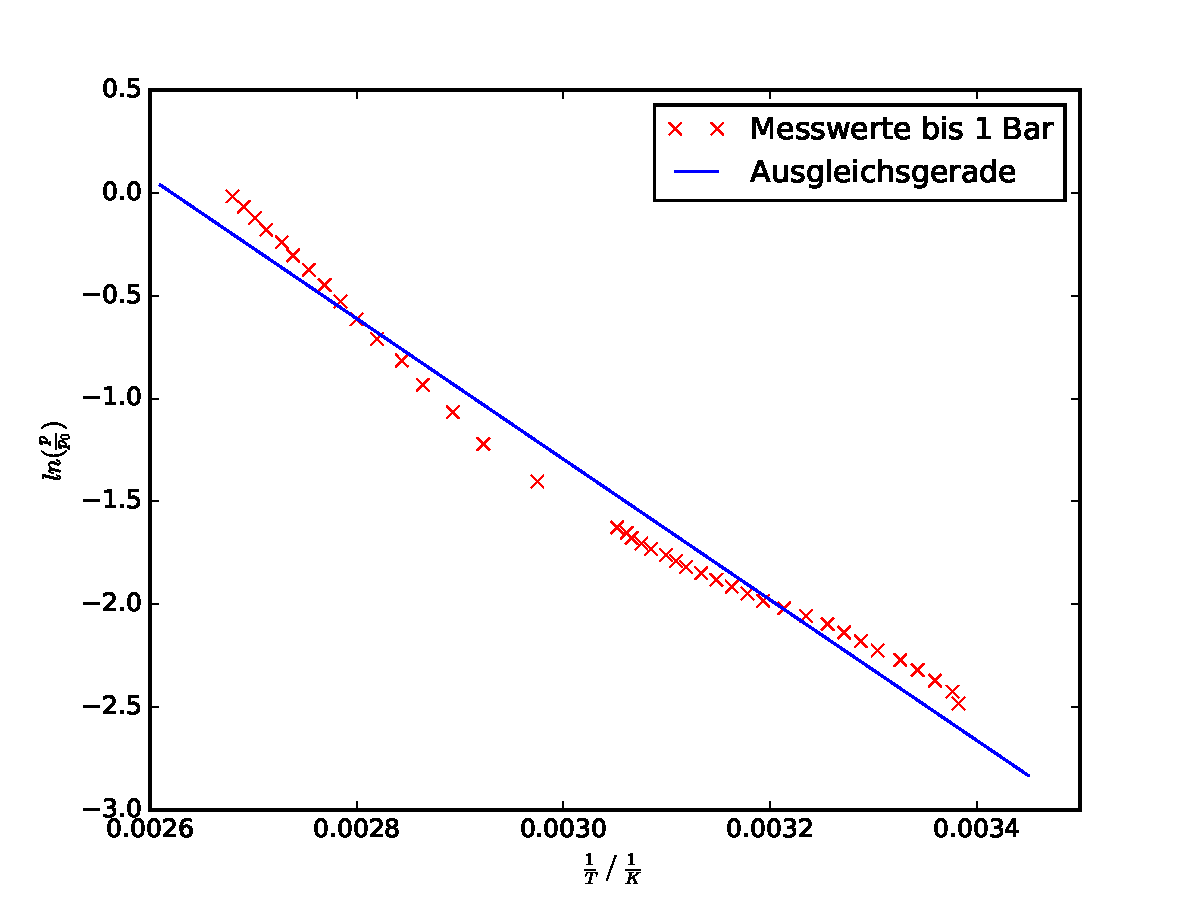
\includegraphics[width=\textwidth]{Plot.pdf}
  \caption{Graph der gemessenen Werte von $ln \left( p \right)$ in Abhängigkeit von der reziproken
  Temperatur $\frac{1}{T}$, mit Ausgleichsgerade.}
  \label{fig:plot1}
\end{figure}\\
Als Steigung erhält man $m = \SI{-3417(86)}{}$ und als Y-Achsenabschnitt $b = \SI{9.0(3)}{}$.\\
Anhand von Formel \eqref{eqn:formel4} folgt für m
\begin{equation}
  m = -\frac{L}{\mathup{R}}
\end{equation}
und damit erhält man $L = \SI{2.84(7)e4}{\joule\per\mol}$.\\

Nun soll $L_a$ abgeschätzt werden. Das ist die Energiemenge, die nötig ist um ein mol des Stoffes von
flüssig zu gasförmig übergehen zu lassen. Also die Arbeit, um das Volumen entsprechend auszudehnen $\left( W = p \cdot V \right)$.
So kann $L_a$ mit der Allgemeinen Gasgleichung abgeschätzt werden. Dies soll nun für eine Temperatur von $\SI{373}{\kelvin}$ getan werden.
\begin{equation}
  L_a = pV = \mathup{R} \, \cdot \, T = \SI{3101.122}{\joule\per\mol}
  \label{eqn:La}
\end{equation}

Um die molekularen Anziehungskräfte bei der Verdampfung zu überwinden ist die Arbeit $L_i$ nötig.
Diese bestimmt man indem man $L_a$ von $L$ abzieht.
\begin{equation}
  L_i = L - L_a = \SI{25311(718)}{\joule\per\mol}
\end{equation}

Das Ergebnis wird durch die Avogadro-Konstante $N_{\mathup{A}}$ \cite{chemav} geteilt und in
Elektronenvolt ($\SI{1}{\electronvolt} = \SI{1.602e-19}{\joule}$) angegeben.
\begin{equation}
  L_i = \SI{0.262(7)}{\electronvolt}
\end{equation}
\subsection{Messung über $\SI{1}{\bar}$}
Anhand dieser Messung soll die Temperaturabhängigkeit der Verdampfungswärme untersucht werden.
Dazu wird Formel \eqref{eqn:formel1} nach L umgeformt.
\begin{equation}
  L = T \left( V_{\mathup{D}} - V_{\mathup{F}} \right) \frac{\symup{d}\,p}{\symup{d}\,T}
  \label{eqn:Lmitabl}
\end{equation}
Um die Ableitung $\frac{\symup{d}\,p}{\symup{d}\,T}$ zu bestimmen, wird zunächst zu den
Wertepaaren ein Ausgleichspolynom 4. Grades bestimmt, wie in dem Graphen \ref{fig:plot2} zu sehen ist.\\
Das Polynom hat dabei die Form:
\begin{equation}
  p \left( T \right) = a \, \cdot \, T^4 + b \, \cdot \, T^3 + c \, \cdot \, T^2 + d \, \cdot \, T + e
  \label{eqn:polynomP}
\end{equation}
Beim Fit mittels Python erhält man dann diese Parameter:\\
\begin{align}
  a &= \SI{2.8(4)e-6}{\bar\per\kelvin\tothe{4}}\\
  b &= \SI{-0.0048(6)}{\bar\per\cubic\kelvin}\\
  c &= \SI{3.1(4)}{\bar\per\kelvin\squared}\\
  d &= \SI{-871(117)}{\bar\per\kelvin}\\
  e &= \SI{92592(12601)}{\bar}
\end{align}
Das Polynom ist dann nach T abzuleiten.\\
\begin{equation}
  \frac{\symup{d}\,p}{\symup{d}\,T} = 4a \, \cdot \, T^3 + 3b \, \cdot \, T^2 + 2c \, \cdot \, T + d
  \label{eqn:dpolynomPdT}
\end{equation}
$V_{\mathup{F}}$ kann immernoch vernachlässigt werden, doch
$V_{\mathup{D}}$ lässt sich nicht mehr mit der Allgemeinen Gasgleichung berechnen.
Stattdessen verwendet man als Näherung:
\begin{align}
  \Bigl( p + \frac{a}{V^2} \Bigr) V &= R \, T &{\mathup{mit}}& &a = \SI{0.9}{\joule\cubic\meter\per\mol\squared}
  \label{eqn:neuVd}
\end{align}
\begin{equation}
  V_{\mathup{D}} = \frac{RT}{2p} \pm \sqrt{\frac{R^2T^2}{4p^2}-\frac{a}{p}}
  \label{eqn:Vd}
\end{equation}
Durch Einsetzen erhält man dann eine Formel für $L \left( T \right)$:
\begin{equation}
  L \left( T \right) = \frac{T}{p} \biggl( \frac{RT}{2} \pm \sqrt{\Bigl( \frac{RT}{2} \Bigr)^{\!\!2} - a \, p} \biggr) \frac{\symup{d}\,p}{\symup{d}\,T}
  \label{eqn:LT}
\end{equation}
Die Verläufe von $L \left( T \right)$ sind in den Graphen \ref{fig:plot3} und \ref{fig:plot4} dargestellt.
\begin{figure}
  \centering
  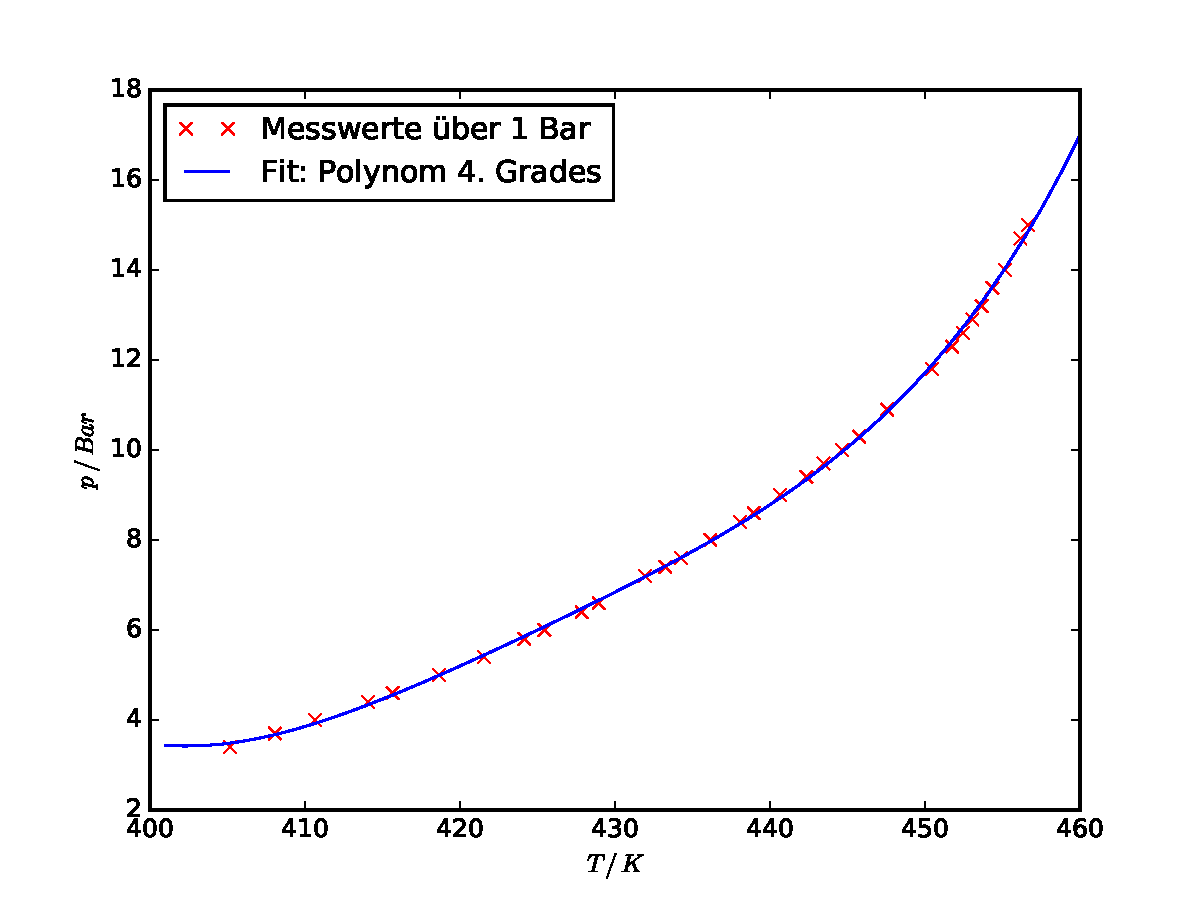
\includegraphics[width=\textwidth]{Plot2.pdf}
  \caption{Gemessene Werte von $p$ in Abhängigkeit von der Temperatur $T$}
  \label{fig:plot2}
\end{figure}
\begin{figure}
  \centering
  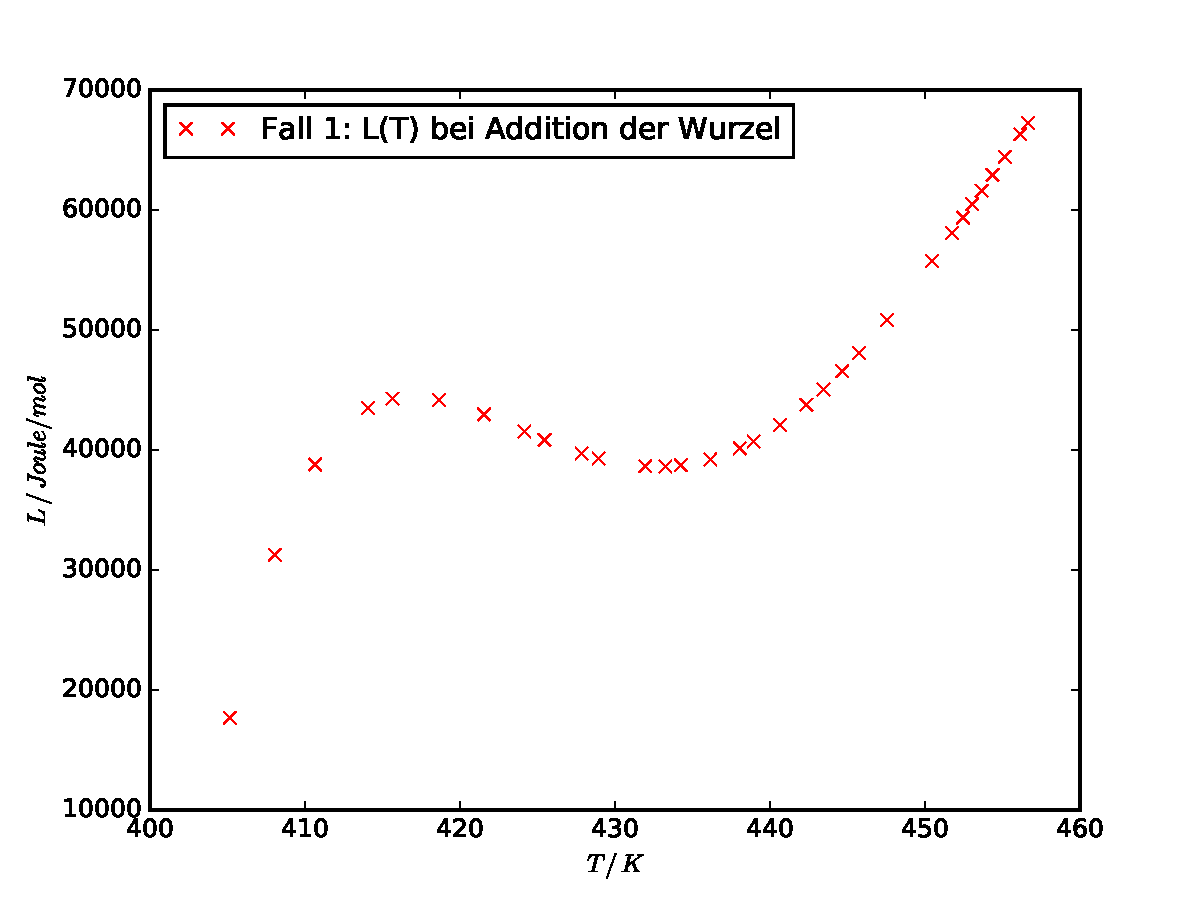
\includegraphics[width=\textwidth]{Plot3.pdf}
  \caption{Verlauf von $L \left( T \right)$ bei Addition der Wurzel}
  \label{fig:plot3}
\end{figure}
\begin{figure}
  \centering
  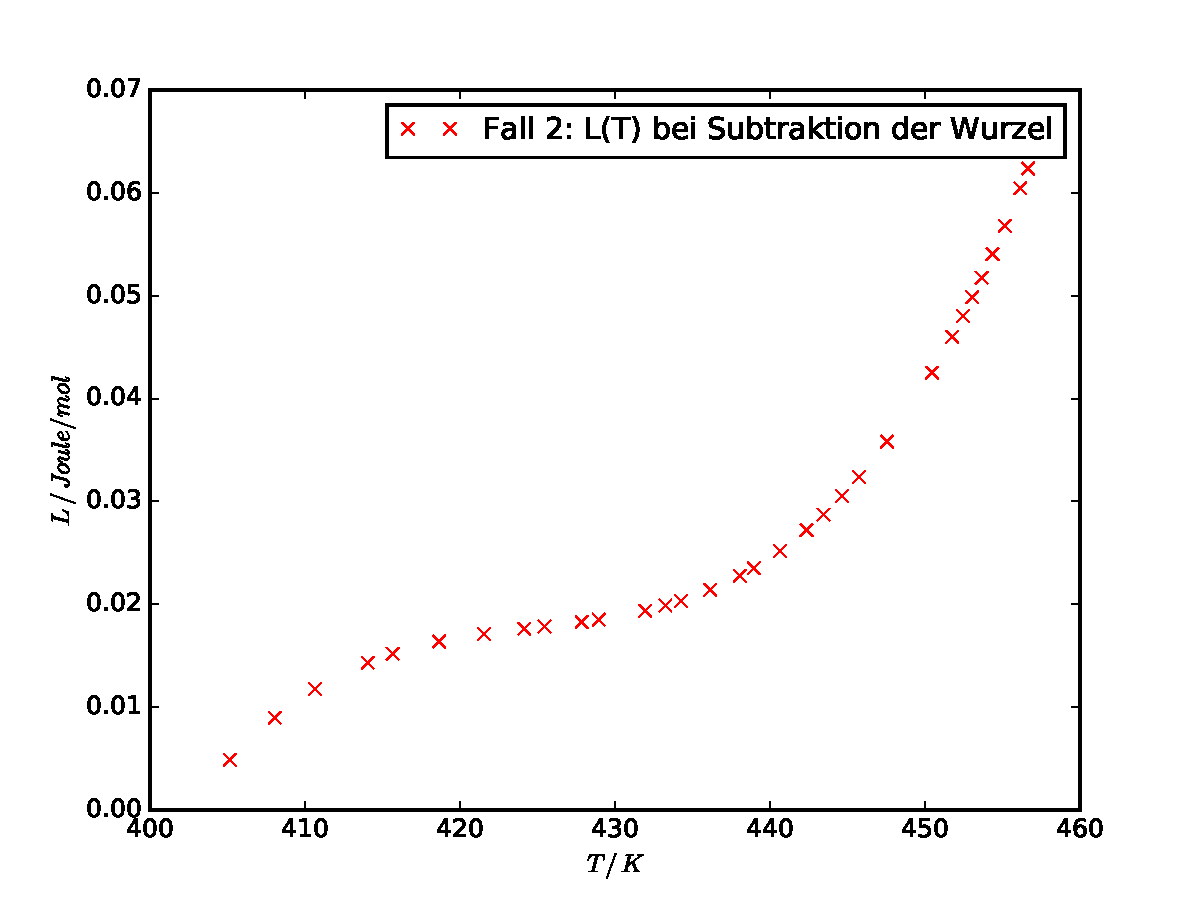
\includegraphics[width=\textwidth]{Plot4.pdf}
  \caption{Verlauf von $L \left( T \right)$ bei Subtraktion der Wurzel}
  \label{fig:plot4}
\end{figure}
\newpage
\begin{table}
  \centering
  \caption{Werte von L(T) für die gemessenen Temperaturen.}
  \label{tab:FunktionswerteL(T)}
  \sisetup{table-format=3.1}
  \begin{tabular}{S[table-format=5.0] S[table-format=2.2] S}
    \toprule
    {Bei Addition der Wurzel} & {Bei Subtraktion der Wurzel} & \\
    {$L \left( T \right) \,/\, \si{\joule\per\mol}$} & {$L \left( T \right) \,/\, \si{\milli\joule\per\mol}$} & {$T \,/\, \si{\celsius}$}\\
    \midrule
    17686 & 4.89 & 132.0\\
    31264 & 8.98 & 134.9\\
    38795 & 11.75 & 137.5\\
    43502 & 14.32 & 140.9\\
    44277 & 15.20 & 142.5\\
    44171 & 16.38 & 145.5\\
    42964 & 17.13 & 148.4\\
    41548 & 17.62 & 151.0\\
    40845 & 17.84 & 152.3\\
    39704 & 18.28 & 154.7\\
    39289 & 18.52 & 155.8\\
    38640 & 19.37 & 158.8\\
    38617 & 19.88 & 160.1\\
    38719 & 20.33 & 161.1\\
    39216 & 21.40 & 163.0\\
    40129 & 22.76 & 164.9\\
    40711 & 23.52 & 165.8\\
    42070 & 25.20 & 167.5\\
    43765 & 27.21 & 169.2\\
    45034 & 28.71 & 170.3\\
    46564 & 30.53 & 171.5\\
    48093 & 32.38 & 172.6\\
    50828 & 35.82 & 174.4\\
    55735 & 42.52 & 177.3\\
    58081 & 46.02 & 178.6\\
    59370 & 48.04 & 179.3\\
    60485 & 49.86 & 179.9\\
    61608 & 51.75 & 180.5\\
    62924 & 54.05 & 181.2\\
    64431 & 56.80 & 182.0\\
    66313 & 60.45 & 183.0\\
    67249 & 62.36 & 183.5\\
    \bottomrule
  \end{tabular}
\end{table}
\newpage
\section{Diskussion}
Als Literaturwert für die Verdampfungswärme von Wasser findet man
$L_{\SI{100}{\celsius}} = \SI{40.8}{\kilo\joule\per\mol}$ \cite{chemst}.
Somit weicht der von uns gemessene Wert um etwa $\frac{1}{3}$ nach unten ab.
Physikalisch macht damit auch nur die Addition der Wurzel in \eqref{eqn:LT} Sinn, wie an den Graphen zu sehen ist.\\
Auffällig ist, dass die von uns bestimmte Abhängigkeit von $L \left( T \right)$ sehr stark steigt, obwohl die
Verdampfungswäre beim kritischen Punkt gegen 0 laufen sollte.
Das könnte aber auch daran liegen, dass der kritische Punkt für Wasser bei einer Temperatur
von $\SI{647.1}{\kelvin}$ und einem Druck von $\SI{221}{\bar}$ liegt \cite{chemth} und dies
nicht in dem von uns betrachteten Bereich liegt. Somit könnte es auch sein, dass sich
jenes Verhalten erst bei höheren Temperaturen einstellt.
Ein weiterer Faktor ist, dass die Wasserstrahlpumpe beim ersten Versuch nur in der Lage
war den Druck auf etwa $\SI{80}{\milli\bar}$ zu senken.
Möglicherweise war die Apparatur auch etwas undicht.
Beim zweiten Versuch stieg die Temperatur sehr schnell, weshalb sich möglicherweise das
Gleichgewicht erst verspätet eingestellt hat. Außerdem war damit das Ablesen etwas schwieriger.
\nocite{*}
\printbibliography

\end{document}
